\chapter{MAV design}
\label{ch:mav-des}
Martian sample return has never been attempted, as a matter of fact a sample return from a celestial body with an atmosphere has never been done before. When designing a sample return missions for Mars, a vital part of it is getting the samples off of the planet. This can then either be send directly to Earth or rendezvous with a \ac{s/c} (either orbiting the planet or not), but either way, the samples have to be able to get there first. This chapter will focus on the different possibilities of \ac{MA} that have already been investigated and/or proposed (\Cref{sec:previnv}) and other (advanced, unconventional or futuristic) ideas for a Martian application described in \Cref{sec:futuidea}. 

%, other conventional techniques that could be considered as well


\section{Previous investigations}
\label{sec:previnv}
Many studies have already been done focused on a \ac{MAV}. A number of these studies have been gathered  and are shown in \Cref{tab:refmavstud}. For each study, the main launch concept is given and the kind of propellant(s) as well. They are presented in order of publication year. 

\begin{table}[!ht]
\begin{center}
\caption{Previous \ac{MAV} studies}
\label{tab:refmavstud}
\begin{tabular}{|p{5cm}|p{5cm}|p{5cm}|}
\hline 
\textbf{Who} 		& \textbf{Which method} & \textbf{Kind of propellant(s)} \\ \hline \hline
J.C. Whitehead \cite{whitehead1997} 		& two stage rockets (comparison study)  & solid and liquid (and gel recommended too)  \\ \hline
C.S. Guernsey \cite{guernsey1998} 		& two stage rocket & 2x liquid  \\ \hline
P.N. Desai et al. \cite{desai1998} 		& two stage rocket & 2x liquid  \\ \hline
C. Stone	\cite{stone1999}	& two stage rocket & hybrid  \\ \hline
D.D. Stephenson \cite{stephenson2002} 		& two stage rocket (three different designs) & 2x Solid (Best), Solid and liquid or hybrid and 2x gel (Best)  \\ \hline
J.C. Whitehead \cite{whitehead2005} 		& one, two and three stage rockets (variational study)  & solid and liquid  \\ \hline
D.D. Stephenson and H.J. Willenberg 		\cite{stephenson2006}& two stage rocket & 2x solid  \\ \hline
A. Sengupta et al. \cite{sengupta2012} 		& two stage rocket & 2x liquid  \\ \hline
M.A. Trinidad et al. \cite{trinidad2012} 		& two stage rocket & 2x liquid  \\ \hline
G. Mungas et al. 	\cite{mungas2012}	& single stage rocket & liquid mono-propellant  \\ \hline
Mars Program Planning Group 	\cite{mppg2012}	& undefined rocket & solid and liquid  \\ \hline
 		
% 		&  &   \\ \hline
\end{tabular}
\end{center}
\end{table} 

From the table it is clear that all studies envision a rocket to bring the samples either into Martian orbit or back to Earth. Also, four clear propellant types have been investigated: the traditional solid and liquid propellant engines, the hybrid engine (which is a combination of a solid fuel and a liquid oxidizer) and the gel engine. The gel engine uses a gel as a propellant. A gel propellant behaves as a viscoelastic solid when stored and burns as a liquid when pressure is applied and the gel is atomized \cite{natan2002}. It was developed as a stable propellant for missiles and the first successful missile was launched in 1999 by \ac{TRW} (now Northrop  Grumman). It is rather important to know the amount of stages and the kind of propellant because that also determines the ascent trajectory and the final orbit the \ac{MAV} can reach. A good overview of stages versus propellants is given by \cite{trinidad2012} (see \Cref{fig:examplestaging_trinidad2012})for a hypothetical scenario where the payload to orbit is 31 $kg$. This table is meant as a comparison for the four different propellant types. 

\begin{figure}[!ht]
\centering
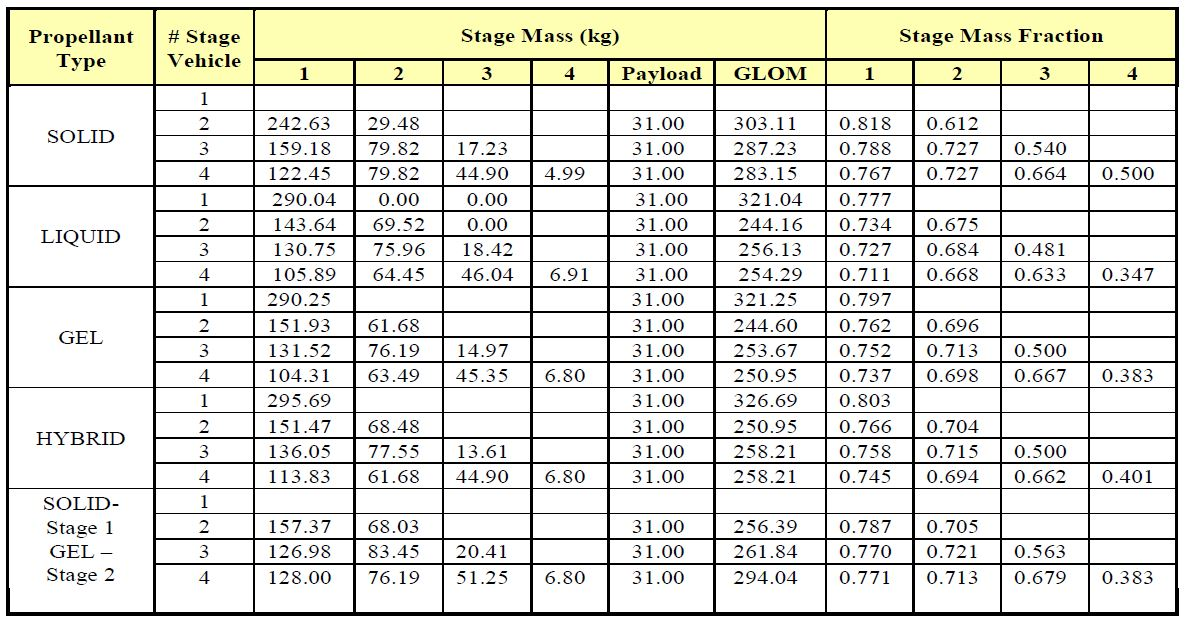
\includegraphics[width=0.9\textwidth]{figures/launcher_methods/examplestaging_trinidad2012.jpg}
\caption{Image of comparison table for different stages with different propellants\cite{trinidad2012}}
\label{fig:examplestaging_trinidad2012}
\end{figure}

This particular study showed that the \ac{GLOM} would be lowest when using a two stage liquid rocket. However,   a two stage gel rocket would be a close second. A low \ac{GLOM} is however not the only requirement which is why at this point no one particular solution can be selected. A visual representation of some of the described designs is given in \Cref{fig:diff_mav_trinidad2012_stephenson2002_mungas2012}.


\begin{figure}[!ht]
\centering
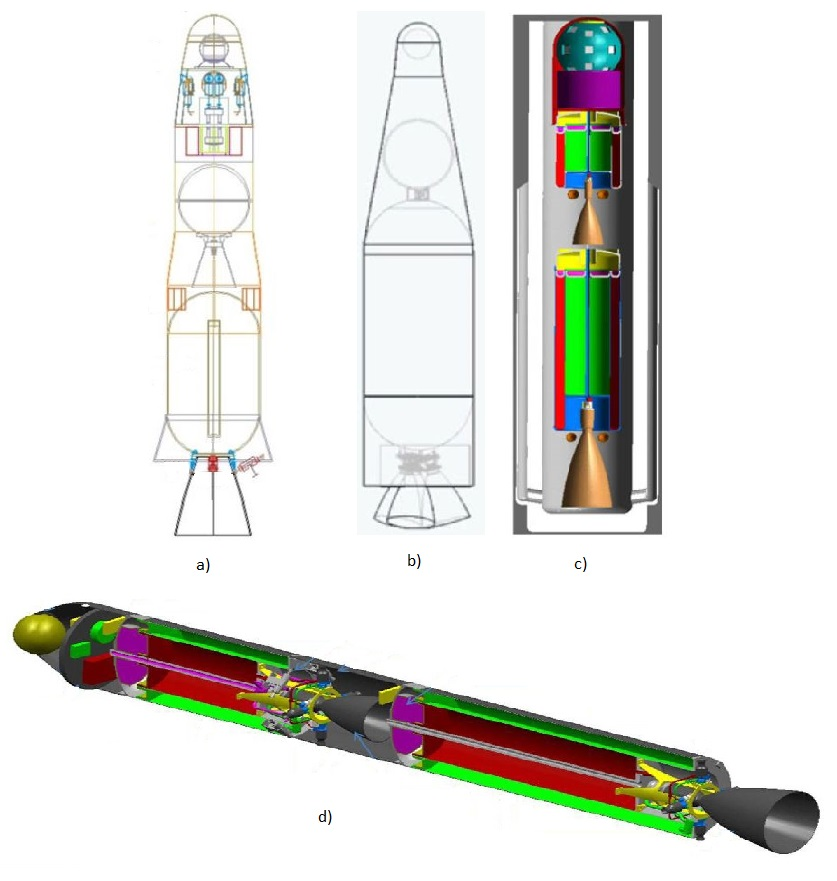
\includegraphics[width=0.4\textwidth]{figures/launcher_methods/diff_mav_trinidad2012_stephenson2002_mungas2012.jpg}
\caption{Some rocket concepts visualized. a) Two stage solid rocket by Lockheed Martin /cite{stephenson2002}, b) Single stage mono-liquid rocket by Firestar Technologies \cite{mungas2012}, c) Two stage gel rocket by \ac{TRW} \cite{stephenson2002} and d) Two stage bi-liquid rocket by Boeing \cite{trinidad2012}}
\label{fig:diff_mav_trinidad2012_stephenson2002_mungas2012}
\end{figure}
  


%\textcolor{red}{\textbf{Also add pictures of some of the proposed systems!!!}}

%\subsection{Solid motor \ac{MAV}}
%\label{subsec:solmav}
%
%
%\subsection{Liquid engine \ac{MAV}}
%\label{subsec:liqmav}
%
%
%\subsection{Hybrid engine \ac{MAV}}
%\label{subsec:hybmav}
%
%\subsection{Gel engine \ac{MAV}}
%\label{subsec:gelmav}
%


\section{Current \ac{MAV} baseline design}
\label{sec:curmavbas}

\section{Current design restrictions}
\label{sec:curdesres}






%\section{Futuristic ideas}
%\label{sec:futuidea}
%Only rockets have been under consideration so far, however other solutions exist as well. These are slightly more exotic and are currently ideas meant for Earth, but it is good to have an overview of everything that is possible.   \Cref{tab:futureover} shows different ideas (order based on publication date) that have been proposed for Earth launches. For all of these systems it should be investigated if and how these methods could be applied on Mars. 
%
%\begin{table}[!ht]
%\begin{center}
%\caption{Futuristic non-rocket launch methods for Earth}
%\label{tab:futureover}
%\begin{tabular}{|p{5cm}|p{10cm}|}
%\hline 
%\textbf{Who} 		& \textbf{Which method}  \\ \hline \hline
%J. Pearson \cite{pearson1975} 		& Space elevator: A counterweight far from Earth would allow a vehicle to travel on a cable between that counterweight and the Earth  \\ \hline
%K.H. Lofstrom 	\cite{lofstrom1985}	& Launch loop: A launch cable that remains stable due to the rotation of the Earth   \\ \hline
%R.H. Frisbee 	\cite{frisbee2003}	&  Microwave propulsion: Based on heat/energy exchange of a ground based microwave generator to heat on-board propellants \\ \hline
%J.T. Kare \cite{kare2004}	&  Laser launch: Based on the heat/energy exchange of a ground laser to heat on-board propellants \\ \hline
%J. Hunter \cite{hunter2012} 	& Space gun: A water based space gun based on rapid gas propulsion  \\ \hline
%Zero2infinity \cite{zero2infinity_2014} 		&  Balloon launch: Balloon carrying rocket and ignited in the stratosphere \\ \hline
%
% 		
%% 		&   \\ \hline
%\end{tabular}
%\end{center}
%\end{table} 
%
%At this point in time most of these systems cannot be applied on Mars because it either involves creating a large infrastructure or demands a lot of energy. However, a balloon launch could be possible and might be worth investigating. 
